% Chapter Template

\chapter{Analysis of cell's properties} % Main chapter title

\label{AppendixA} % Change X to a consecutive number; for referencing this chapter elsewhere, use \ref{ChapterX}


In this appendix, the distributions of symbolic features are analyzed. The histogram of values for each symbolic features is plotted with regard to class.


%----------------------------------------------------------------------------------------
%	FEATURES
%----------------------------------------------------------------------------------------

\begin{figure}
	\begin{center}
		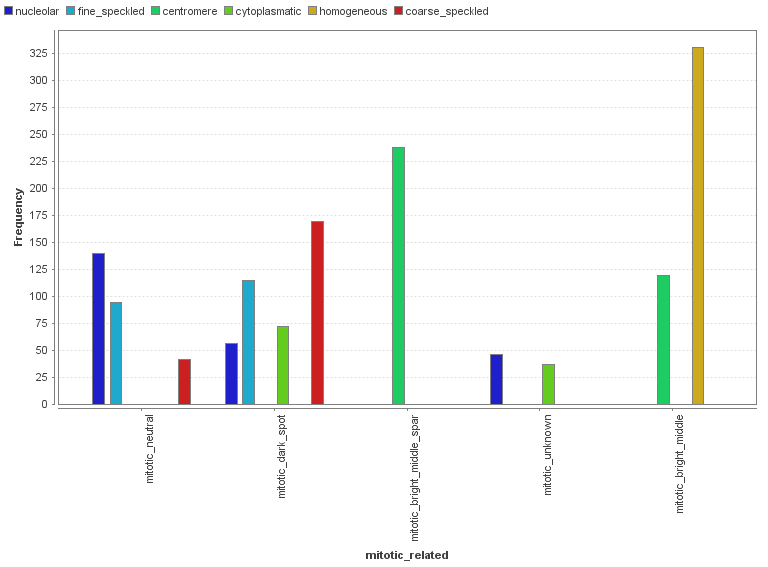
\includegraphics[width=14cm, height=8cm]{Figures/AppendixA/mitotic_related}
		\caption{The histogram showing how different types of mitotic cells relate to patterns}
	\end{center}
\end{figure}

\begin{figure}
	\begin{center}
		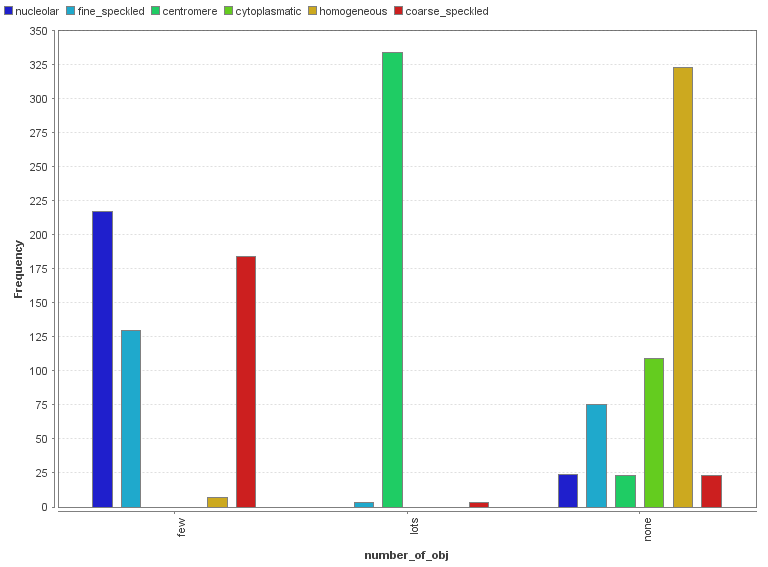
\includegraphics[width=14cm, height=9cm]{Figures/AppendixA/number_of_organelles}
		\caption{The histogram showing how many organelles each pattern express}
	\end{center}
\end{figure}

\begin{figure}
	\begin{center}
		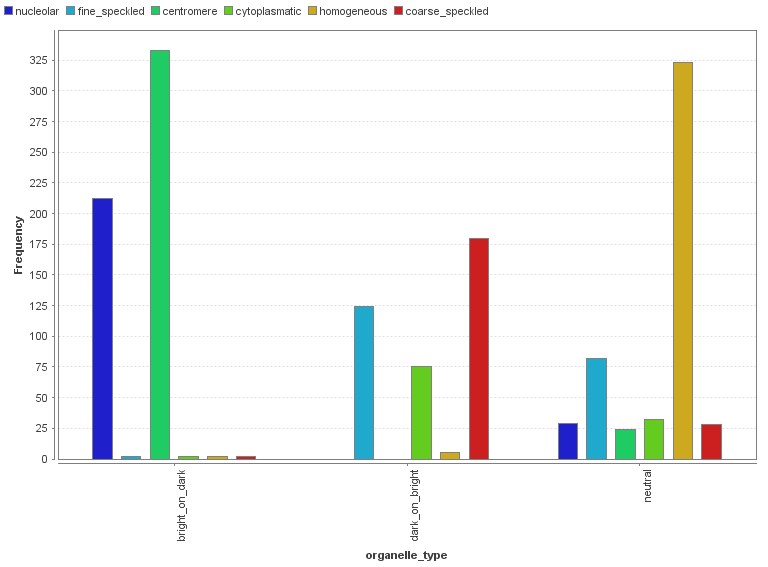
\includegraphics[width=14cm, height=9cm]{Figures/AppendixA/organelle_type}
		\caption{The histogram showing which kind of organelles could be found in certain patterns}
	\end{center}
\end{figure}

\begin{figure}
	\begin{center}
		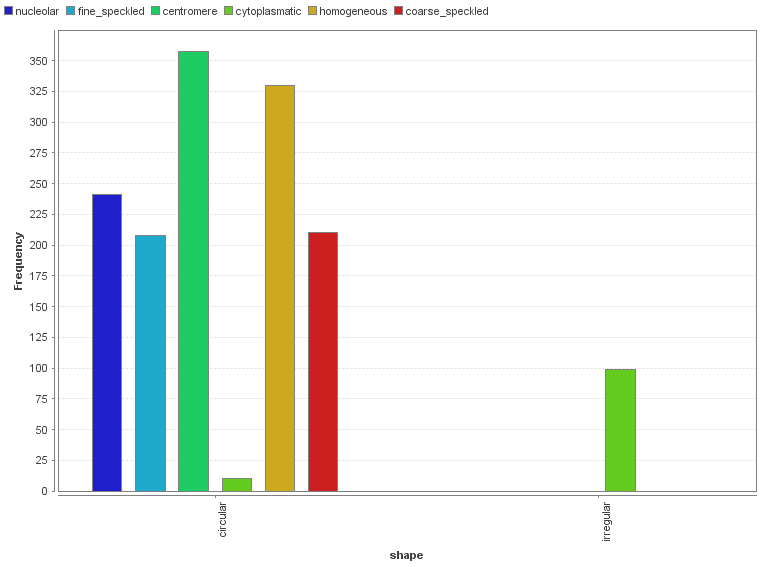
\includegraphics[width=14cm, height=9cm]{Figures/AppendixA/shape}
		\caption{The histogram showing which shape patterns expose}
	\end{center}
\end{figure}